 
Для рассмотрения резонансного случая удобно перейти в систему координат Делоне, в которой гамильтониан имеет вид \cite{plummer}:
$$H = - \frac{(1-\nu)^2}{2L^2} - \nu R(L, \rho_1, \rho_2, l, \omega_1, \omega_2),$$
где возмущающая функция $R$ равна:
$$R = \sum_{s-j-k+p-m-n=0, s \geq 0} K^{sjkpmn}(L, \rho_1, \rho_2) \cos(s l + p l_J + j \omega_1 + k \omega_2 + m \omega_{1J} + n \omega_{2J}).$$
Здесь $(1-\nu)$ - масса Солнца, $\nu \approx \frac{1}{1000}$ - масса Юпитера, являющаяся малым параметром. Все углы, относящиеся к Юпитеру, обозначены индексом $J$, а углы, связанные с астероидом, обозначаются без индекса, гравитационная постоянная полагается равной единице. В терминах эллиптических элементов переменные выражаются формулами:
$$L = \sqrt{(1-\nu)a},$$
$$\rho_1 = \sqrt{(1-\nu)a}(1-\sqrt{1-e^2}),$$
$$\rho_2 = \sqrt{(1-\nu)a(1-e^2)}(1-\cos i),$$
здесь $a$ - большая полуось, $e$ - эксцентриситет, $i$ - наклон орбиты, $l$ - средняя долгота, $\omega_1$ - долгота перицентра, $\omega_2$ - долгота восходящего узла.

\begin{figure}[htp]
\centering
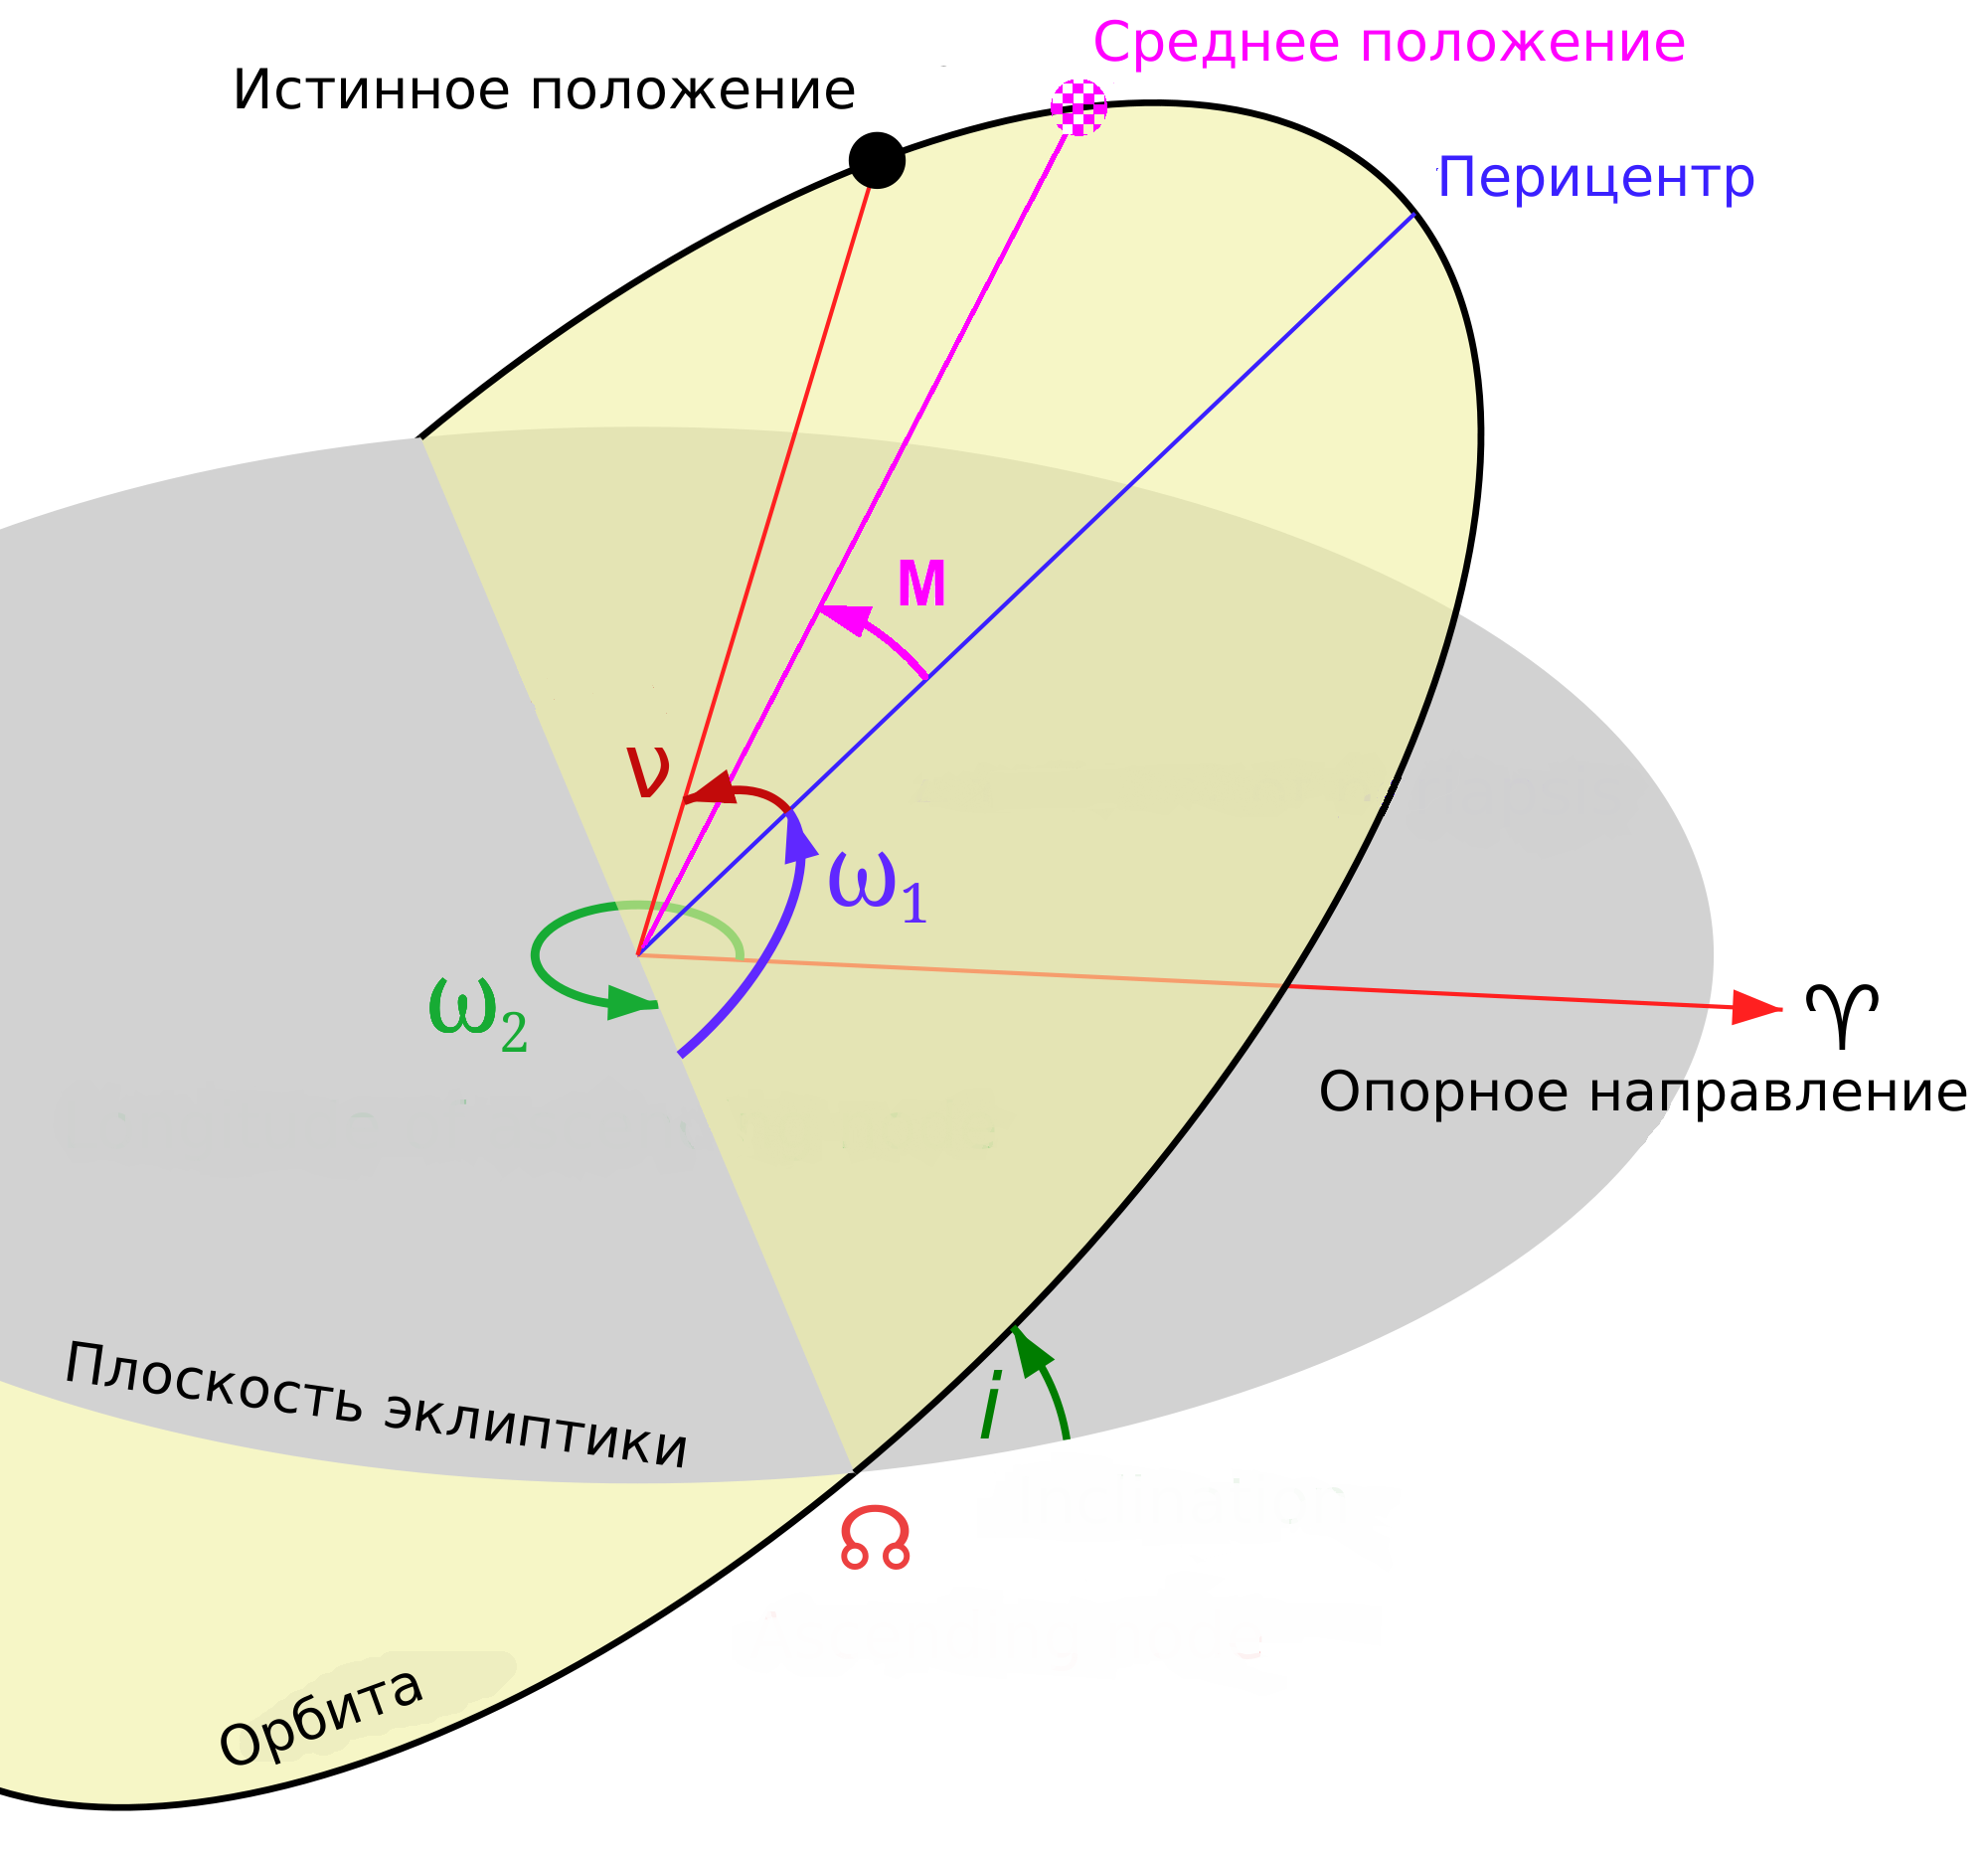
\includegraphics[scale=0.12]{../img/Orbit1-mean.png}
\caption{Средняя долгота $l = \omega_1 + \omega_2 + M$, где $M$ - средняя аномалия}
\end{figure}

Резонанс возникает когда аргументы косинусов близки к стационарным \cite{wis2}:
$$s l + p l_J + j \omega_1 + k \omega_2 + m \omega_{1J} + n \omega_{2J} = \text{const}.$$

Учитывая, что средняя долгота $l$ меняется значительно быстрее остальных углов, получаем резонансное условие (точка обозначает производную по времени):
$$s \dot l + p \dot l_J \approx 0, $$
которое можно переписать в виде:
$$\dot l \approx \frac{-p}{s} \dot l_J \equiv \frac{s+q}{s} \dot l_J.$$

Число $q$ называется порядком резонанса и для исследуемого в данной работе резонанса 3:1 $q=2$, $s=1$.

Учтем, что рассматривается плоская задача, следовательно, $i=0$, $\rho_2=0$, $\omega_2=0$. Подставляя известные коэфициенты ряда и отбрасывая все члены старше второго порядка по $e_J$, получаем \cite{wis2}:
$$H = - \frac{(1-\nu)^2}{2L^2} - \nu R_{sec}(\rho_1, \omega_1) - \nu R_{res}(L,l,\rho_1,\omega_1),$$
где $R_{sec}(\rho_1, \omega_1) = - 2 \rho_1 F - e_J G \sqrt{2 \rho_1} \cos \omega_1$ - секулярная часть возмущающей функции, содержащая медленно меняющиеся со временем члены и в общем случае не периодические, 

$R_{res}(L,l,\rho_1,\omega_1) = 2 \rho_1 C \cos(l-\omega_1-3 l_J)+e_J^2E \cos(l - 3 l_J)$ - резонансная часть возмущающей функции, содержащая медленно изменяющиеся периодические члены.

Масштабным преобразованием можно добиться  \cite{wis2}:
$$a_J=1, \dot l_J= 1 .$$

Производя замену:
$$\Lambda = L - L_{res},$$
$$\lambda = l - 3 l_J,$$
$$x = \sqrt{2 \rho_1} \cos \omega_1,$$
$$y = \sqrt{2 \rho_1} \sin \omega_1,$$
и раскладывая гамильтониан по степеням $\Lambda$, получаем в старшем порядке:
\begin{equation}
\label{Ham_res}
H = \alpha \frac{\Lambda^2}{2} + \nu \left( C(x^2-y^2)+e_J D x + e_J^2 E \right) \cos \lambda + \nu (2Cxy+e_J D y) \sin \lambda + \nu e_J G x + \nu F(x^2+y^2),
\end{equation}
где $L_{res} = \left( \frac{(1-\nu)^2}{3} \right)^\frac13$ - центр резонанса, определяемый условием резонансности 
$$
\dot \lambda = \frac{\partial H}{\partial L}|_{L=L_{res}}=0,$$
a постоянная $\alpha$: 
$$\alpha = -\frac{3(1-\nu)^2}{L_{res}^4} < 0.$$

Следует отметить, что $y$ и $\lambda$ являются координатами, а $x$ и $L$ сопряженными к ним импульсами. При этом фазовое пространство рассматриваемой системы  четырехмерно и, учитывая периодичность правой части уравнений по $\lambda$, можно считать, что:
$$(x,y,\Lambda,\lambda) \in \mathbb{R}^3 \times S^1 .$$

Коэфициенты $F,G,C,D,E,e_J$ являются известными константами, значения которых в случае системы Солнце-Юпитер можно найти, например, в \cite{wis1}.

Систему, описываемую гамильтонианом (\ref{Ham_res}), принято называть плоской эллиптической ограниченной задачей трех тел в случае главного резонанса 3:1.